\chapter{Getting started}                % Print a "chapter" heading
This chapter describes how to work with virtualized environments that contain pre-configured simulation packages. There are several such packages available. Each contains an implementation of the Medical Simulation Markup Language (MSML) as well as different simulation backends. In the following we describe how to run these environments based on Docker containers\footnote{\url{www.docker.com} }. We also describe how to connect to server instances that run dockerized MSML environments.   
 
\section{Running MSML-based Docker containers}
In this section, we describe how to run a pre-configured deployment of the Simulation Open Framework Architecture (SOFA) simulation package. 

\subsection{Installing the container}                  % Print a "section" heading

\begin{enumerate}
	\item Install the Docker framework for your Linux distribution. Further details can be found on the Docker homepage. For Ubuntu Linux there is the possibility to use either pre-configured packages (see \url{www.ubuntuupdates.org/ppa/docker} or to install Docker manually (\url{http://docs.docker.com/installation/ubuntulinux/}).
	\item Optional: You can add your user to the docker group in order to avoid the use ofsudo in front of the docker commands:
		\begin{lstlisting}[language=sh]
  $ sudo usermod -aG docker username
\end{lstlisting}
Please remember to log out in order to for the changes to take effect.
	\item Pull the SOFA container from the Docker Hub: 
	\begin{lstlisting}[language=sh]
  $ docker pull ssuwelack/msml_sofa
\end{lstlisting}
\end{enumerate}

\subsection{Running the container} 

There are two different options to run a graphical application inside the simulation container:
\begin{enumerate}
	\item Start an SSH server inside the container and connect to it. This typically is a very stable set-up, but introduces an additional overhead.
	\item Link the host X-server into the container. This approach can achieve bare metal performance, if the native graphics drivers are part of the container. However, it does not work on all host systems and has problems with Qt-based apps.	
\end{enumerate}

In the following we describe how to start the container in each mode. The start-up procedures described below are available in script form from Github:
 \begin{lstlisting}[language=sh, breaklines=true]
  $ git clone https://github.com/ssuwelack/msml-docker-runtime.git
\end{lstlisting}

\subsubsection{Communicating to the container over SSH (recommended)}

\begin{enumerate}
 \item The following command starts the Docker container as a daemon, assigns it the name msml\_sofa and binds it's SSH port to port 22000 of the localhost:
	\begin{lstlisting}[language=sh, breaklines=true]
  $ docker run -d -p 127.0.0.1:22000:22 --name msml_sofa ssuwelack/msml_sofa /root/start_ssh.sh 
\end{lstlisting}

\item Alternatively, the startup script can be used:
	\begin{lstlisting}[language=sh, breaklines=true]
  $ ./start_ssh_msml_sofa.sh
\end{lstlisting}

\item We can use the pre-configured user msml (password: msml) to connect to the running container using SSH:
	\begin{lstlisting}[language=sh]
  $ ssh -XC msml@localhost -p 22000
\end{lstlisting}

\item The sofa runtime is located at /opt/sofa/bin. All data is stored in the home directory of the msml user.

\item The container can be stopped by executing
\begin{lstlisting}[language=sh, breaklines=true]
  $ docker stop msml_sofa
\end{lstlisting}
on the host machine. It can be re-started using the command
\begin{lstlisting}[language=sh, breaklines=true]
  $ docker start msml_sofa
\end{lstlisting}
Stopped containers can be deleted through
\begin{lstlisting}[language=sh, breaklines=true]
  $ docker rm msml_sofa
\end{lstlisting}

\end{enumerate}

\subsubsection{Communicating to the container via X-server sockets}

In order to run the container with minimally overhead, the X-server socket can be forwarded. A start-up script is available in the above mentioned repository that carries out the necessary steps:
\begin{lstlisting}[language=sh, breaklines=true]
  $ ./run_msml_sofa.sh
\end{lstlisting}



\section{Connecting to a server instance}  
 
In order to avoid the work of setting up individual environments, the containers can be run on a server instance. In order to connect to such a container, you need the following information:
\begin{itemize}
	\item Server name
	\item Public port number of the container
	\item Jump host name (if server is protected by a firewall)
	\item If not changed by the container provider, login credentials are: 
	
	\begin{description}
		\item[User: msml] 
		\item[Password: msml] 
	\end{description}
	
\end{itemize}

\subsection{Connecting from a Linux client}

In order to connect from a linux clients, just run:
	\begin{lstlisting}[language=sh]
  $ ssh -XC msml@servername -p portnumber
\end{lstlisting}

\subsection{Connecting from a Windows client}

The MobaXterm framework can be used to connect from a windows machine.
 In this section, we describe how to run SOFA on a server instance. The server i61sv002.ira.uka.de exposes 25 docker container that run SOFA from port 22001 to 22025. In order to access these containers from a Linux machine inside the the HIS network, simply run
	\begin{lstlisting}[language=sh, breaklines=true]
  $ ssh -XC msml@i61sv002.ira.uka.de -p 22010
\end{lstlisting}

In the following we describe how the containers can be accessed from any Windows machine.

\begin{enumerate}
	\item Install the MobaXterm framework which you can download on its homepage (http://mobaxterm.mobatek.net/download-home-edition.html).
	\item Open MobaXterm and start a new session (cf. figure \ref{mobaXtermNewSession}).
	\item Configure your SSH session (cf. figure \ref{mobaXtermSessionConfig}):
		\begin{itemize}
 			 \item server name
 			 \item user / password (standard is msml/msml)
 			 \item port number
 			 \item jump host for port forwarding and login credentials for jump host
		\end{itemize}	
\end{enumerate} 

\begin{figure}[h]
  	\centering
    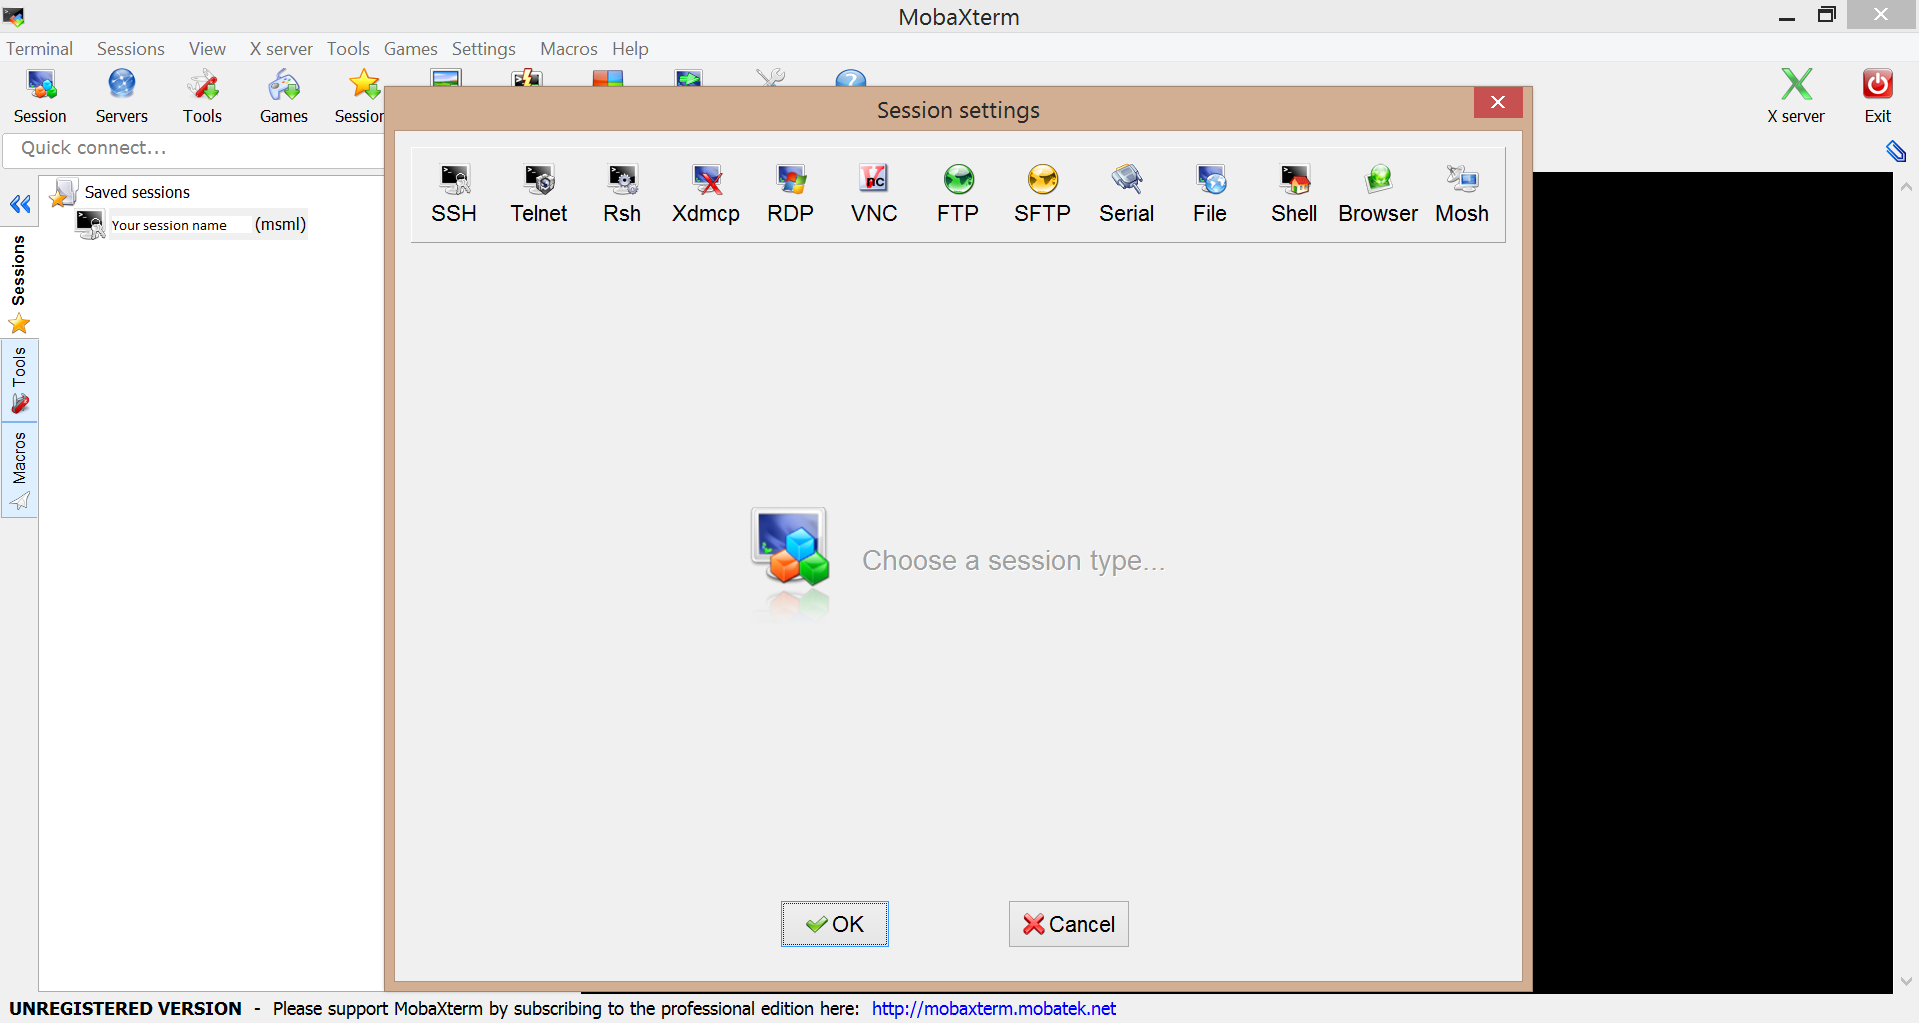
\includegraphics[width=\textwidth]{pictures/MobaXterm_newSession}
    \caption{Screenshot of MobaXterm after starting a new session.}
    \label{mobaXtermNewSession}
\end{figure}

 
\begin{figure}[h]
  	\centering
    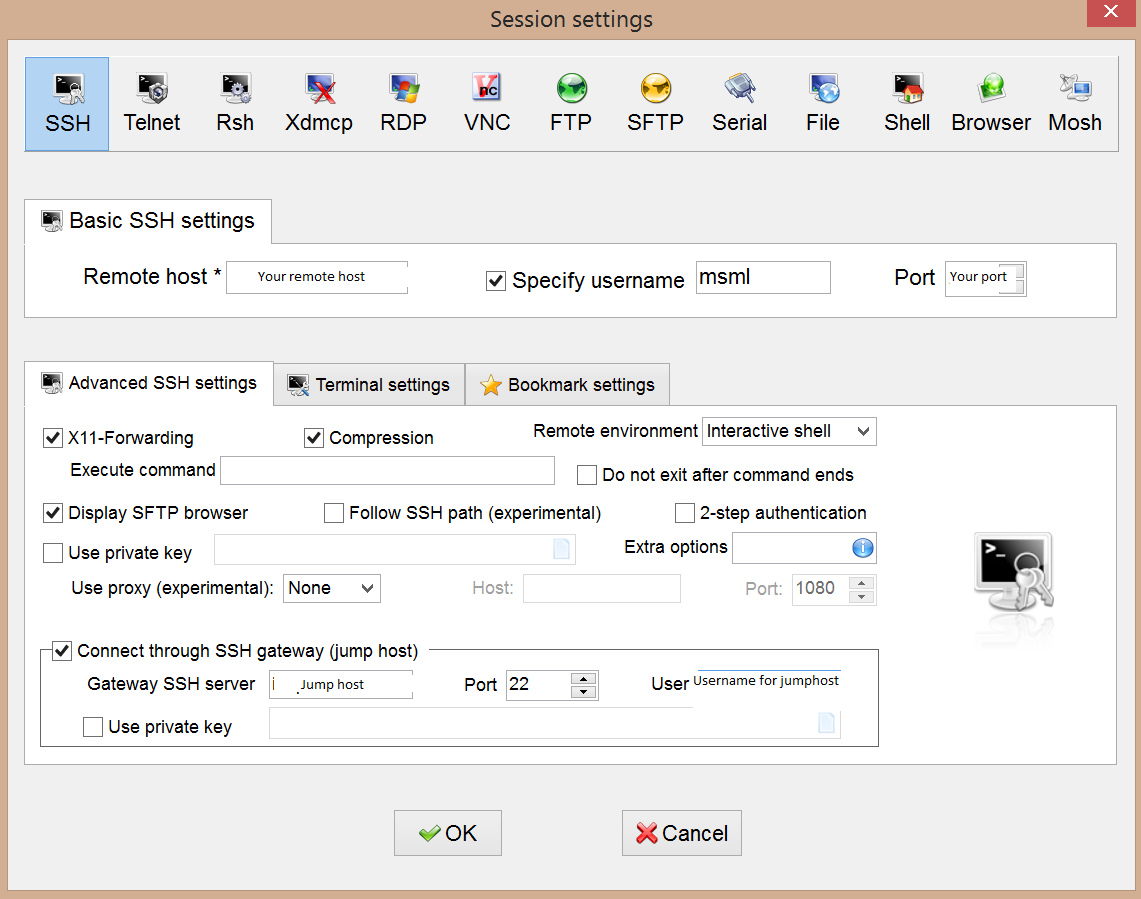
\includegraphics[width=\textwidth]{pictures/MobaXterm_SessionConfig}
    \caption{Screenshot of MobaXterm after starting a new session.}
    \label{mobaXtermSessionConfig}
\end{figure}

 
%\section{Own Installation}
%\label{sec:own-installation}
%
%If you need better OpenGL support or more speed, you should install SOFA and MSML by yourself. This process takes a couple of time for installing several dependencies and  compiling. You should calculate with two or three hours, depending on your system performance.
%
%\subsection{SOFA Installation}
%\label{sec:sofa-installation}
%
%Start by getting the latest SOFA version\footnote{More detail: \url{https://wiki.sofa-framework.org/wiki/Getting_Started}}. 
%
%\begin{lstlisting}[language=sh, breaklines=true]
%git clone --depth 1 git://scm.gforge.inria.fr/sofa/sofa.git
%\end{lstlisting}
%For the compilation you need to install following packages (Ubuntu): 
%\begin{lstlisting}[language=sh, breaklines=true]
%sudo apt-get install cmake cmake-qt-gui cmake-curses-gui ccache \
%build-essential libqt4-dev libglew-dev\
%freeglut3-dev libpng-dev zlib1g-dev\
%python2.7-hdev libxml2-dev libcgal-dev libblas-dev\
%liblapack-dev libsuitesparse-dev \
%libboost-all-dev libassimp-dev 
%\end{lstlisting}
%
%Create a new folder, go into it, and trigger CMake. 
%
%\begin{lstlisting}[language=sh, breaklines=true]
%mkdir sofa-build
%cd sofa-build
%cmake ../sofa
%cmake ../sofa 
%make -j 8
%\end{lstlisting}
%
%\subsection{MSML}
%
%MSML consists of two parts: C++ functionality and a Python core.  
%First, check out the MSML repository:
%
%\begin{lstlisting}[language=sh, breaklines=true]
%git clone --depth 1 https://github.com/CognitionGuidedSurgery/msml.git
%\end{lstlisting}
%
%
%For C++ we need several libraries (Ubuntu):
%
%\begin{lstlisting}[language=sh, breaklines=true]
%sudo apt-get install libtet1.5-dev libcgal-dev libvtk6-dev \
%libxml2-dev  
%libboost-filesystem-dev libboost-python-dev \
%libboost-program-options-dev libboost-graph-dev \
%libboost-iostreams-dev \
%python-vtk6 swig python-pip 
%\end{lstlisting}
%
%The CMake build process takes care about everything else.
%
%\begin{lstlisting}[language=sh, breaklines=true]
  %mkdir msml-build
  %cd msml-build
  %cmake ../msml/operators
  %make -j 8
%\end{lstlisting}
%
%The Python dependencies are installed via pip:
%
%\begin{lstlisting}[language=sh, breaklines=true]
%pip install -r msml/requirements.txt
%\end{lstlisting}
%
%
%
%
%%%% Local Variables:
%%%% mode: latex
%%%% TeX-master: "../SoftTissueSimulationBook"
%%%% End:
